\documentclass{beamer}
\usetheme{Dresden}
\usepackage[spanish]{babel}
\usepackage[utf8]{inputenc}

\begin{document}
\title{Ciclo completo de CI/CD con Dagger y Kubernetes}
\subtitle{Grado en Ingeniería Informática \\
    Universidad de Santiago de Compostela}
\author{Autor: Daniel Vieites Torres}
\institute{Tutor: Juan Carlos Pichel Campos \\ Co-tutor: Francisco Maseda Muiño}
\date{15 de septiembre de 2025}

\begin{frame}
    \titlepage
\end{frame}

\section{Contexto}

\subsection{CI/CD}
\begin{frame}
    \frametitle{CI/CD}
    \begin{figure}
        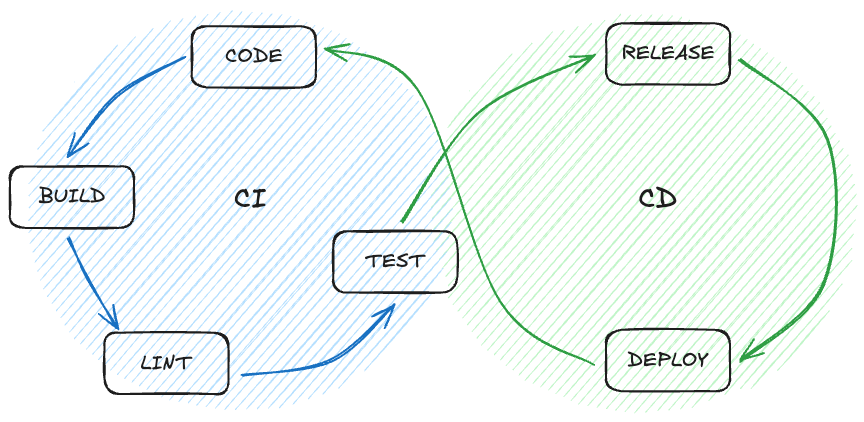
\includegraphics[scale=0.35]{figuras/ci_cd}
        \caption{Ciclo de CI/CD de este TFG.}
    \end{figure}
\end{frame}

\subsection{El problema}
\begin{frame}
    \frametitle{¿Cuál es el problema?}
    \begin{columns}
        \begin{column}{0.45\textwidth}
            \begin{itemize}
                \item<1-> Aplicaciones con un gran volumen de tecnologías.
                \item<2-> Gran complejidad.
                \item<3-> Coste de mantenimiento elevado.
            \end{itemize}
        \end{column}
        \begin{column}{0.55\textwidth}
            \begin{figure}
                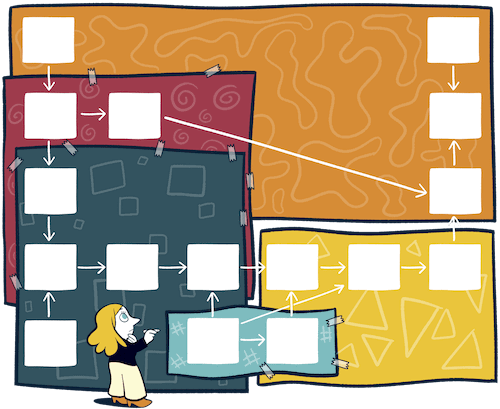
\includegraphics[scale=0.33]{figuras/complejidad}
            \end{figure}
        \end{column}
    \end{columns}
\end{frame}

\subsection{La solución}

\begin{frame}
    \frametitle{¿Qué se propone?}
    \begin{figure}
        
\includegraphics[scale=1.2]{figuras/Dagger_logo}
    \end{figure}
    \begin{center}
        {\it Dagger} para gestionar CI/CD.
    \end{center}
\end{frame}

\begin{frame}
    \frametitle{Dagger}
    \begin{columns}
        \begin{column}{0.45\textwidth}
            \begin{itemize}
                \item<1-> SDK de creación de \textit{pipelines} de CI/CD.
                \item<2-> Múltiples lenguajes.
                \item<3-> Módulos.
                \item<4-> {\it Runtime} de OCI.
                \item<5-> Uso de caché.
            \end{itemize}
        \end{column}
        \begin{column}{0.55\textwidth}
            \begin{figure}
                \includegraphics<1>[scale=0.2]{figuras/dagger}
                \includegraphics<2>[scale=0.25]{figuras/languages}
                \includegraphics<3>[scale=0.4]{figuras/daggerverse}
                \includegraphics<4>[scale=0.4]{figuras/docker}
                \includegraphics<5>[scale=0.1]{figuras/cache}
                \only<5>{\caption{Imagen generada con IA.}}
            \end{figure}
        \end{column}
    \end{columns}
\end{frame}

\section{Organización}
\begin{frame}
    \frametitle{Organización de GitHub}
    \begin{figure}
        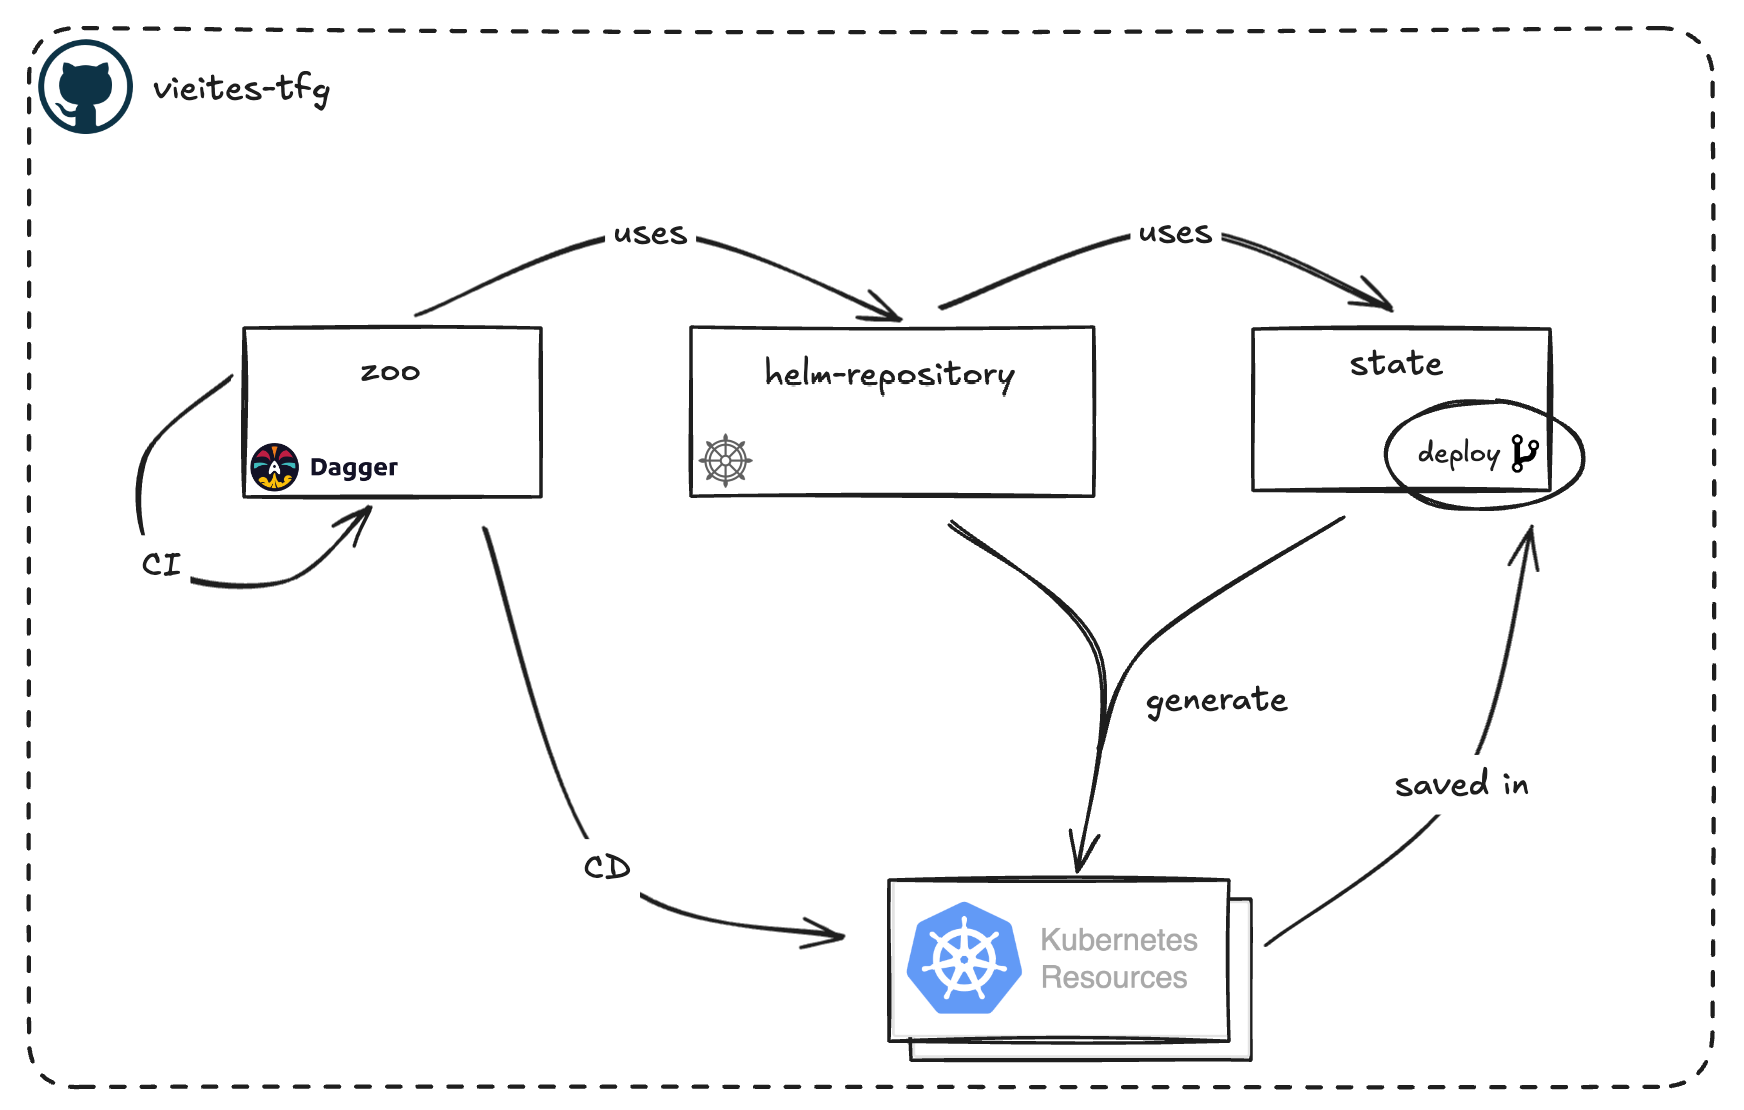
\includegraphics[scale=0.28]{figuras/vieites-tfg}
    \end{figure}
\end{frame}

\section{CI}
\subsection{App}
\begin{frame}
    \frametitle{Zoo}
    \begin{figure}
        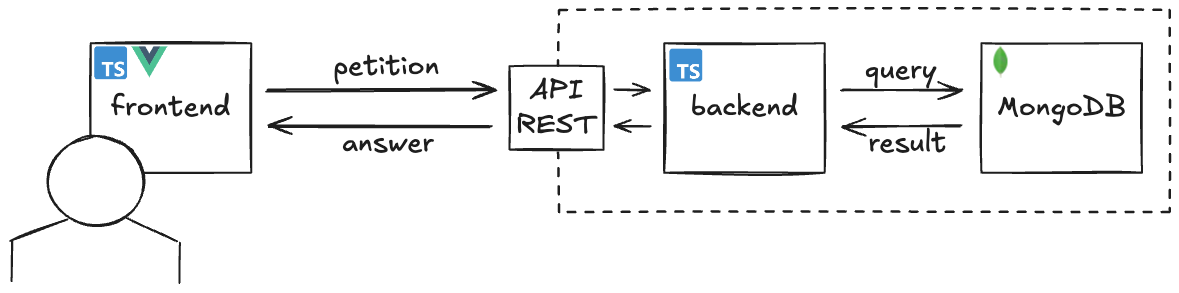
\includegraphics[scale=0.25]{figuras/app}
        \caption{Elementos de la aplicación.}
    \end{figure}
\end{frame}

\subsection{CI con Dagger}
\begin{frame}
    \frametitle{CI con Dagger}
    \begin{figure}
        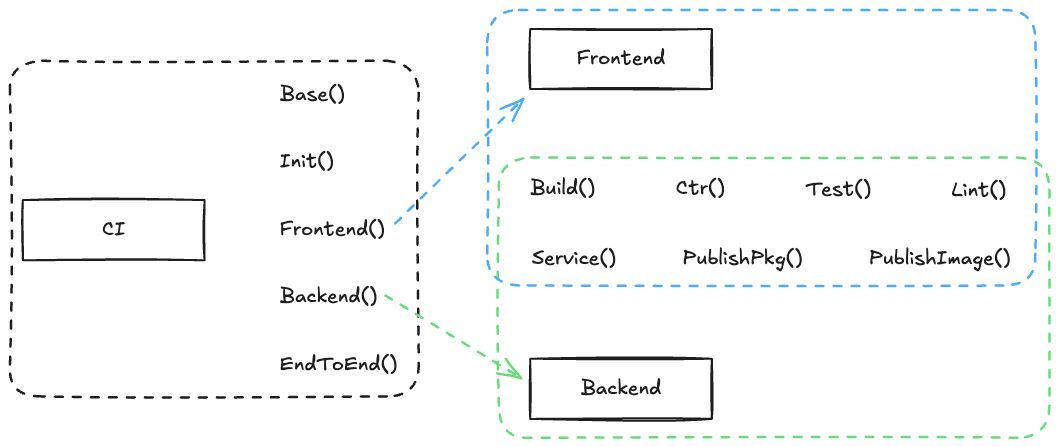
\includegraphics[width=10.8cm]{figuras/ci_dagger_go}
        \caption{Estructura del módulo de CI con Go.}
    \end{figure}
\end{frame}

\section{CD}
\subsection{Estructura de despliegue}
\begin{frame}
    \frametitle{helm-repository}
    \begin{figure}
        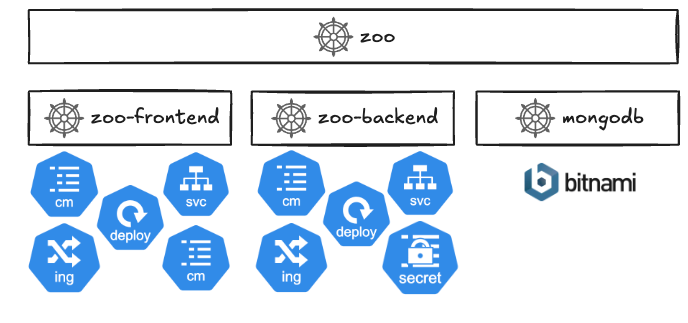
\includegraphics[scale=0.4]{figuras/helm-repository}
        \caption{Estructura de despliegue de la aplicación.}
    \end{figure}
\end{frame}

\begin{frame}
    \frametitle{state}
    \begin{figure}
        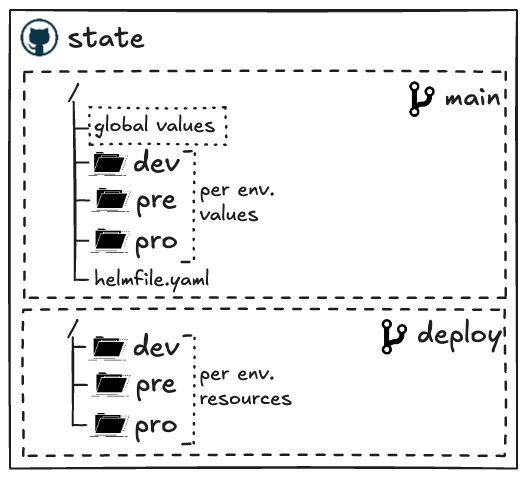
\includegraphics[scale=0.3]{figuras/state}
        \caption{Estructura del repositorio de estado.}
    \end{figure}
\end{frame}

\begin{frame}
    \frametitle{GitOps \& ArgoCD}
    \begin{figure}
        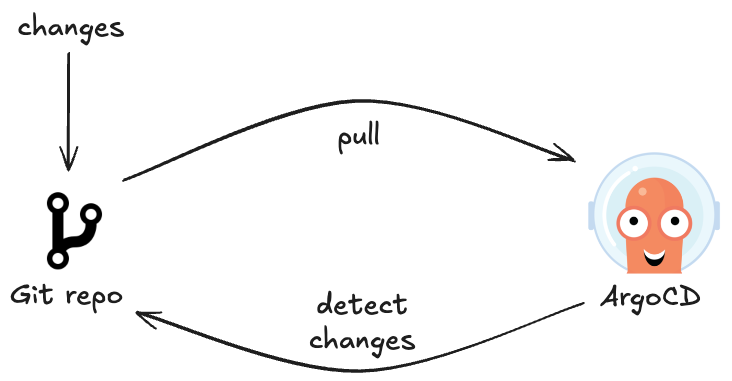
\includegraphics[scale=0.35]{figuras/argocd-simple}
        \caption{Funcionamiento de ArgoCD con GitOps.}
    \end{figure}
\end{frame}

\begin{frame}
    \frametitle{Diferentes entornos}
    \begin{figure}
        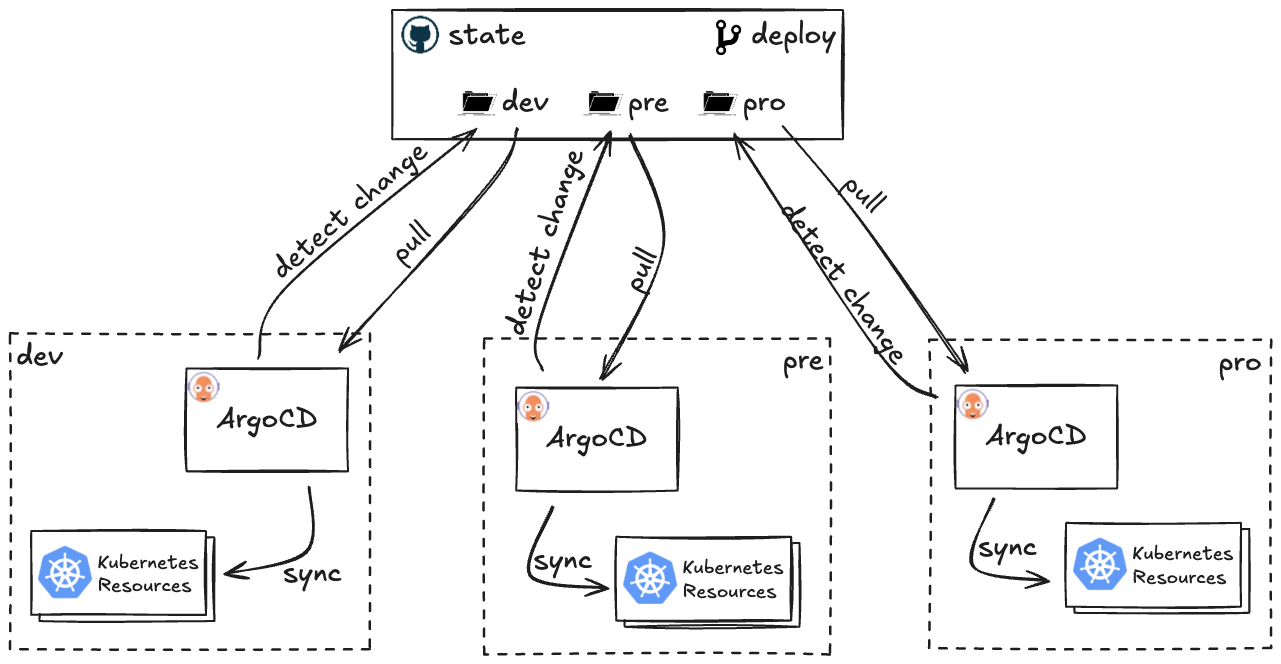
\includegraphics[width=9cm]{figuras/clusters}
        \caption{Un cluster por entorno con ArgoCD instalado.}
    \end{figure}
\end{frame}

\subsection{CD con Dagger}
\begin{frame}
    \frametitle{CD con Dagger}
    \begin{figure}
        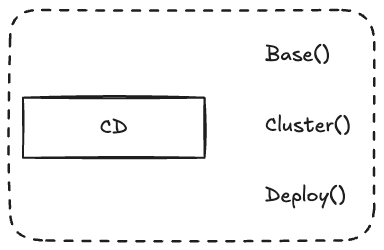
\includegraphics[width=6cm]{figuras/cd_dagger_go}
        \caption{Estructura del módulo de CD con Go.}
    \end{figure}
\end{frame}

\section{Ciclo completo}
\begin{frame}
    \frametitle{Ciclo completo con Dagger}
    \begin{figure}
        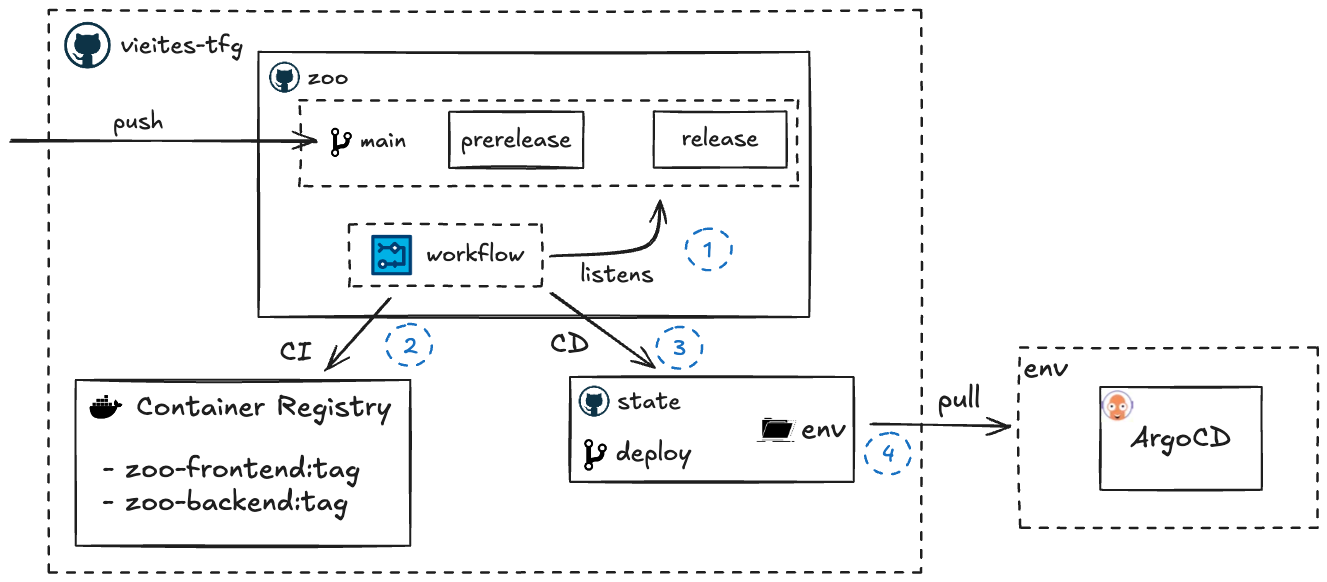
\includegraphics[width=10.8cm]{figuras/promotion}
        \caption{Estructura del módulo de CI/CD con Go.}
    \end{figure}
\end{frame}

\section{Conclusiones}
\begin{frame}
    \frametitle{Rendimiento}
    \begin{figure}
        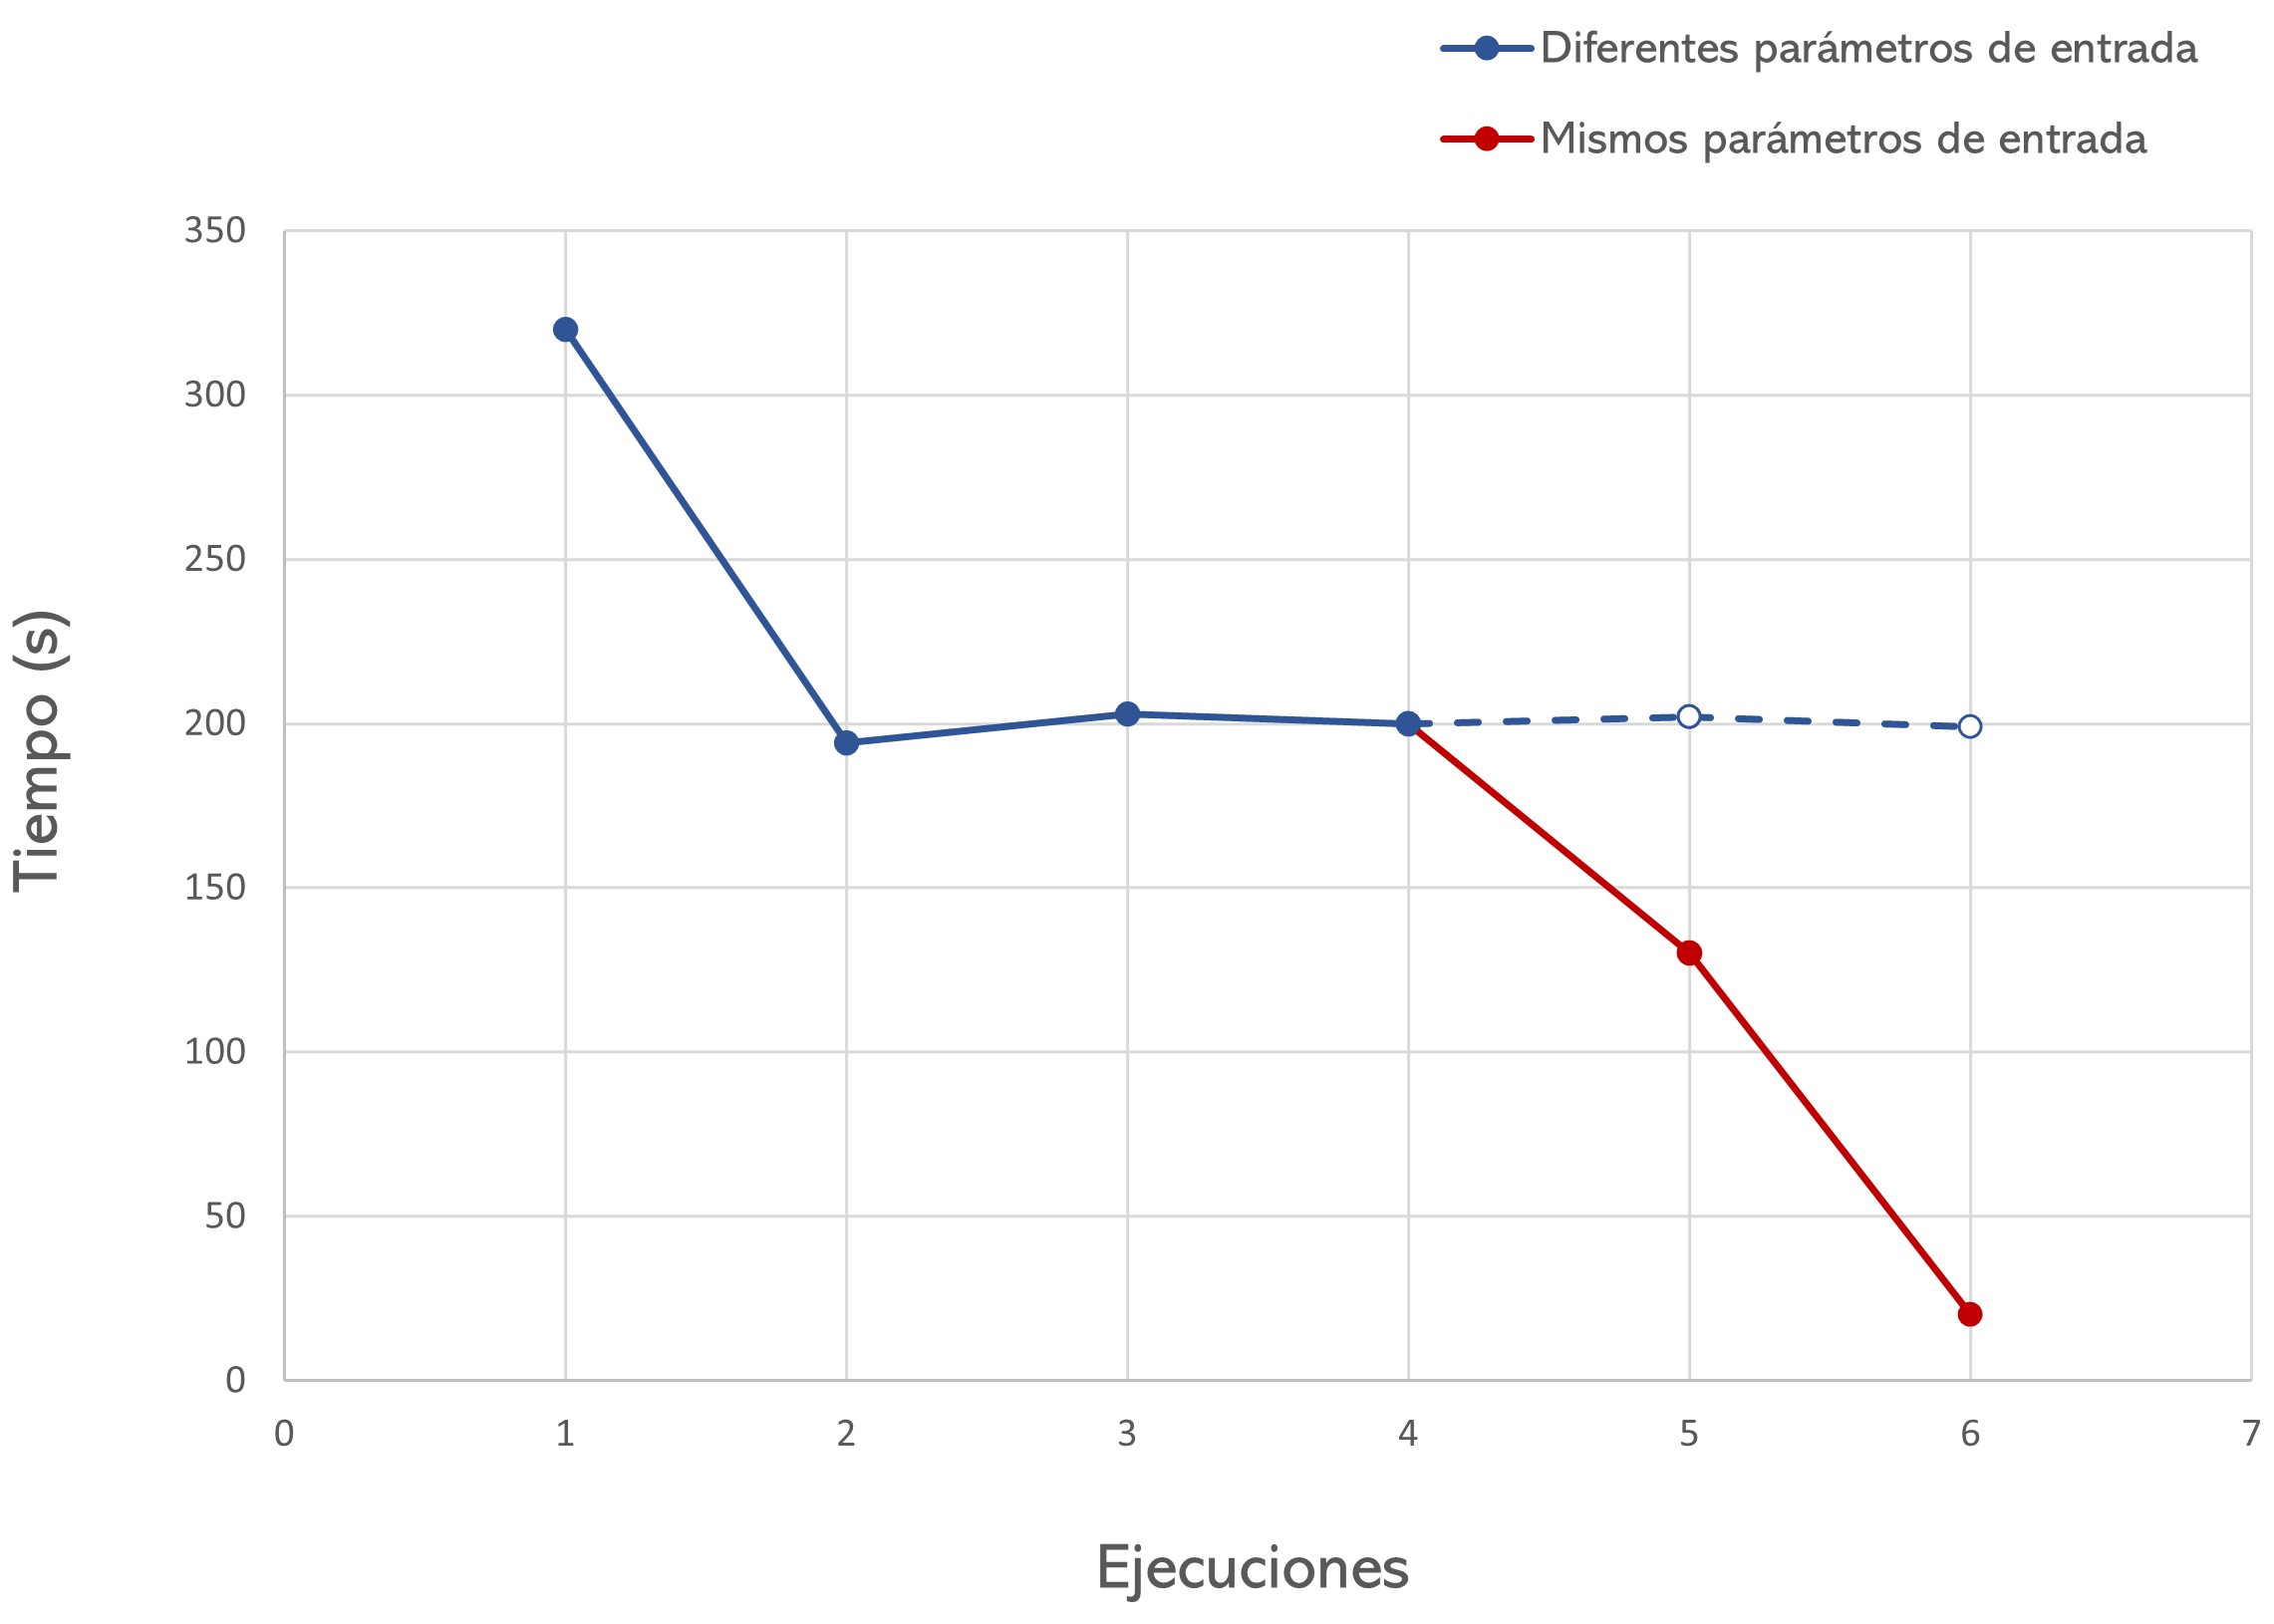
\includegraphics[scale=0.52]{figuras/graph-times}
    \end{figure}
\end{frame}

\begin{frame}
    \frametitle{Conclusiones finales}
    \begin{itemize}
        \item Curva de aprendizaje moderada.
        \item Facilidad de gestión de la lógica de programación.
        \item Mantenimiento a largo plazo.
        \item Gran portabilidad.
        \item Gestión de caché.
        \item Existencia de módulos públicos.
    \end{itemize}
\end{frame}

\section*{}
\begin{frame}
    \titlepage
\end{frame}

\end{document}
